\section{Improving Convergence Speed}
\label{sec:convergence}

A good optimization algorithm is esential for fitting a deep neural network, however the convergence rate can often be improved by modifying the network aritecture itself such that the cost function is easier to optimize. These modifications does not radically alter the network, but rather modifies existing layers. The modifications can also become the idendity function though parameter optimization and thus doesn't change the theoretical capabilities of the neural network.

\subsection{Batch Normalization}
Traditionally in feed forward neural networks it has been the norm to standarize the input to have zero mean and unit variance.
\begin{equation}
\hat{x}_i = \frac{x_i - \mathbb{E}[x_i]}{\sqrt{\textsc{Var}[x_i]}}, \quad \forall i \in [1, I]
\end{equation}

This standaridization places the input to the sigmoid activation function in its linear domain ($\sigma(\epsilon) \approx \epsilon, \forall \epsilon \in [-1, 1]$), which is a reasonable starting point for the optimization \todo{[LeCun et al., 1998b; Wiesler \& Ney, 2011]}. Batch normalization extends this idea to standardize before all activation functions in a deep neural network. This has positive consequences beound limiting the sigmoid activation to its linear domain \cite{batch-normalization}.

Consider a neural network with just one hidden layers:
\begin{equation}
\mathcal{L}(\mathbf{t}, \mathbf{W}_2 \theta(\mathbf{W}_1 \mathbf{x} + \mathbf{b}_1) + \mathbf{b}_2)
\end{equation}
When optimizing the loss function, the parameters $\mathbf{W}_1, \mathbf{W}_2, \mathbf{b}_1$ and $\mathbf{b}_2$ are all optimized simultaneously. Futhermore the optimization of $\mathbf{W}_2, \mathbf{b}_2$ does directly depend on $\theta(\mathbf{W}_1 \mathbf{x} + \mathbf{b}_1)$ though the error term. This becomes and issue when the distribution of $\theta(\mathbf{W}_1 \mathbf{x} + \mathbf{b}_1)$ changes, because the updated $\mathbf{W}_2$ and $\mathbf{b}_2$ assumes the original distribution. This change of the distribution of the internal activations is called an \textit{internal covariate shift}. \cite{batch-normalization}.

The \textit{internal covariate shift} issue can be ilustrated by considering a scalar $a = w x + b \sim \mathcal{N}(b, w)$, as it would appear in a very simple neural network, the sigmoid activation function is the applied on $\mathcal{N}(b, w)$ by using the \textit{change of variable theorem}. Using this one can change $w$ and $b$ and observe how the sigmoid activation distribution changes (Figure \ref{fig:convergence:batch-norm:activation-distribution}).

\begin{figure}[h]
	\centering
	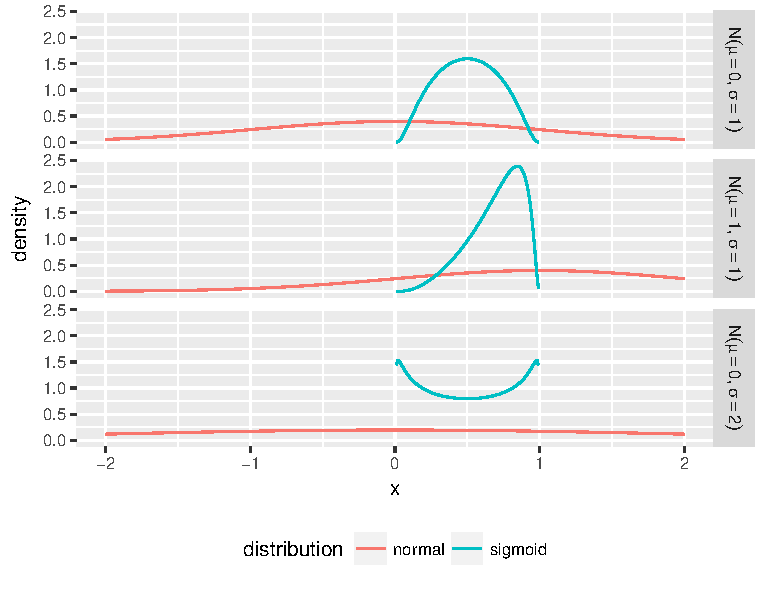
\includegraphics[scale=1]{theory/batch-norm-activation-distribution}
	\caption{Shows $X \sim \mathcal{N}(\mu, \sigma)$ and $\mathrm{sigmoid}(X)$ calculated using the \textit{change of variable theorem}.}
	\label{fig:convergence:batch-norm:activation-distribution}
\end{figure}

\subsubsection{A solution}
The \textit{internal covariate shift} issue can in practis be solved by using a small learning rate, however this is not an optimal solution as it prolongs the optimization. Batch Normalization is an alternative solution, that solves the issue by standardizing the input to the activation function. To truly standardize this input the convariance matrix, as well as its inverse square root should be calculated, this is very expensive thus Batch Normalization makes a pratical compromise by only standardizing using the variance.
\begin{equation}
\hat{z}_{h_\ell} = \frac{z_{h_\ell} - \mathbb{E}[z_{h_\ell}]}{\sqrt{\textsc{Var}[z_{h_\ell}]}}, a_{h_\ell} = \theta(\hat{z}_{h_\ell})
\end{equation}

The expectation ($\mathbb{E}[z_{h_\ell}]$) and variance ($\textsc{Var}[z_{h_\ell}]$) themself are expensive to estimate over the entire dataset, thus it's only done over each mini-batch. This also makes it much more feasable to integrate the standardization into the backward pass. Note also that because the expectation is substracted, the bias $b_{h_\ell}$ in $z_{h_\ell}$ has no effect and should thus be obmitted:
\begin{equation}
z_{h_\ell} = \sum_{h_{\ell-1}}^{H_{\ell-1}} w_{h_{\ell-1}, h_\ell} a_{h_{\ell-1}} 
\end{equation}


Finally to allow Batch Normalization to become the indendity function, two more parameters ($\gamma, \beta$) are added to the optimzation problem:
\begin{equation}
\hat{z}_{h_\ell} = \gamma_{h_\ell} \frac{z_{h_\ell} - \mathbb{E}[z_{h_\ell}]}{\sqrt{\textsc{Var}[z_{h_\ell}]}} + \beta_{h_\ell}, a_{h_\ell} = \theta(\hat{z}_{h_\ell})
\label{eq:theory:convergence:batch-norm}
\end{equation}

The backward pass for learning ($w, \gamma, \beta$) is rather complicated, but computationally completely feasible as long as the mini-batch size is small. See Appendix \ref{appendix:backward-pass:batch-norm} for the backward pass.

In the special case that $\theta(\cdot)$ is multiplicative linear with respect to a scalar (i.e. $\theta(\alpha \hat{z}_{h_\ell}) = \alpha \theta(\hat{z}_{h_\ell})$) and the following layer isn't sensitive to a multplication factor, then $\gamma_{h_\ell}$ can be removed from the optimization. A common case is where $\theta(\cdot)$ is the ReLU function, in this case:
\begin{equation}
\begin{aligned}
\alpha_{h_\ell} = \mathrm{ReLU}(\hat{z}_{h_\ell}) &= \gamma_{h_\ell} \mathrm{ReLU}\left(\frac{z_{h_\ell} - \mathbb{E}[z_{h_\ell}]}{\sqrt{\textsc{Var}[z_{h_\ell}]}} +  \frac{1}{\gamma_{h_\ell}}\beta_{h_\ell}\right)\\
&= \gamma_{h_\ell} \mathrm{ReLU}\left(\frac{z_{h_\ell} - \mathbb{E}[z_{h_\ell}]}{\sqrt{\textsc{Var}[z_{h_\ell}]}} +  \tilde{\beta}_{h_\ell}\right)
\end{aligned}
\end{equation}

In the next layer $\alpha_{h_\ell}$ is then multiplied by some other weight that $\gamma_{h_\ell}$ can be merged into. This simplification can often be applied and can be quite valuable as it removed some computations and futher simplifies the loss curvature.

\subsubsection{Inference}

With an establised backward pass, the network can esily be trained. However there is still an open question about how inference should be done.

The inference should be determinstic once training is done, thus the ideal solution would be to use the estimated expectation and variance from the entire training dataset in \eqref{eq:theory:convergence:batch-norm}. However because this calculation can be rather expensitve a more practial solution is to use a moving average. Lets denote $\sigma^2_{\mathcal{B}_i}$ and $\mu_{\mathcal{B}_i}$ as the variance and mean estimate after mini-batch $i$. Then in addition to the optimization of ($w, \gamma, \beta$), $\sigma^2_{\mathcal{B}_i}$ and $\mu_{\mathcal{B}_i}$ will also updated during training.
\begin{equation}
\begin{aligned}
\sigma^2_{\mathcal{B}_i} &= \lambda \sigma^2_{\mathcal{B}_{i-1}} + (1 - \lambda) \textsc{Var}[z_{h_\ell}] \\
\mu_{\mathcal{B}_i} &= \lambda \mu_{\mathcal{B}_{i-1}} + (1 - \lambda) \mathbb{E}[z_{h_\ell}]
\end{aligned}
\end{equation}

At inference $\hat{z}_{h_\ell}$ are then calculated using $\sigma^2_{\mathcal{B}_i}$ and $\mu_{\mathcal{B}_i}$.

\begin{equation}
\hat{z}_{h_\ell} = \gamma_{h_\ell} \frac{z_{h_\ell} - \mu_{\mathcal{B}_i}}{\sqrt{\sigma^2_{\mathcal{B}_i}}} + \beta_{h_\ell}, a_{h_\ell} = \theta(\hat{z}_{h_\ell})
\end{equation}

\subsubsection{Weight sharing network}

Because it is the weight changes that causes an \textit{internal covariate shift}, the normalization should happen over all $z_{h_\ell}$ values that uses these weights. Thus in RNN the normalization should also be done over time, and in CNN the normalization should also happen over the ``image''. This works well for actual images, however in RNN and CNN that describes a causal relation, the mean and variance at any time step (e.g. $t=0$) will contain information from all time steps, which breaks the causalily of the network. This issue can be practially solves by not normalizing over time, however if the sequences aren't all of the same length then the mean and variance estimation for the last time step will be extremely poor.

\subsection{Layer Normalization}

Layer normalization attemps to solve the issues that exists when Batch Normalization is applied to causal weight shareing networks. It does this by not normalization over the batch, but normalizing over the $\{z_{h_\ell}\}_{h_\ell=1}^{H_\ell}$ vector. \cite{layer-normalization}

\begin{displayquote}
Notice that changes in the output of one layer will tend to cause highly correlated changes in the summed inputs to the next layer, especially with ReLU units whose outputs can change by a lot. This suggests the “covariate shift” problem can be reduced by fixing the mean and the variance of the summed inputs within each layer. \todo{understand this}
\end{displayquote}

Normalizing over the summed inputs $z_{h_\ell}$ results in the following forward pass:
\begin{equationbox}[H]
Activation:
\begin{equation*}
\begin{aligned}
z_{h_\ell} &= \sum_{h_{\ell-1}}^{H_{\ell-1}} w_{h_{\ell-1},h_\ell} a_{h_\ell-1} \\
\hat{z}_{h_\ell} &= \gamma_{h_\ell} \frac{z_{h_\ell} - \mu_{\ell}}{\sqrt{\sigma_{\ell}^2 + \epsilon}} + \beta_{h_\ell} \\
a_{h_\ell} &= \theta\left(z_{h_\ell}\right)
\end{aligned}
\end{equation*}
Statistics:
\begin{equation*}
\begin{aligned}
\mu_{\ell} &= \frac{1}{H_\ell} \sum_{h_\ell}^{H_\ell} z_{h_\ell} \\
\sigma_{\ell}^2 &= \frac{1}{H_\ell} \sum_{h_\ell}^{H_\ell} (z_{h_\ell} - \mu_{\ell})^2
\end{aligned}
\end{equation*}
\caption{Forward equations for Layer Normalization.}
\end{equationbox}

Note that the bias $b_{h_\ell}$ is excluded here for a different reason than what was the case in Batch Normalization. In Batch Normalization $b_{h_\ell}$ was a constant, and is thus removed when the mean is substacted. In Layer Normalization the mean is over $h_\ell \in [1, H_\ell]$ and thus $b_{h_\ell}$ is no longer a constant. However the orignal reasoning for Layer Normalization ``output of one layer will tend to cause highly correlated changes in the summed inputs'', does not include $b_{h_\ell}$ in ``summed inputs'' and thus the normalization should only happen over $\sum_{h_{\ell-1}}^{H_{\ell-1}} w_{h_{\ell-1},h_\ell} a_{h_\ell-1}$. As such $\hat{z}_{h_\ell}$ actually becomes
\begin{equation*}
\hat{z}_{h_\ell} = \gamma_{h_\ell} \frac{z_{h_\ell} - \mu_{\ell}}{\sqrt{\sigma_{\ell}^2 + \epsilon}} + b_{h_\ell} + \beta_{h_\ell},
\end{equation*}
but $ b_{h_\ell}$ then becomes redudant because of $\beta_{h_\ell}$.

The backward pass for learning ($w, \gamma, \beta$) is like in batch normalization a bit complicated, see Appendix \ref{appendix:backward-pass:batch-norm} for the backward pass.

Like in batch normalization the $\hat{z}_{h_\ell}$ calculation can be simplified if $\theta(\cdot)$ is scalar multiplicative linear (i.e. $\theta(\alpha \hat{z}_{h_\ell}) = \alpha \theta(\hat{z}_{h_\ell})$) and $\gamma_{h_\ell}$ can be merged into a weight in the following layer.

\subsubsection{Properties}

Batch Normalization and Layer Normalization have somewhat similar properties, as shown in Table \ref{table:convergence:layer-norm:properties}. \textit{Weight matrix re-centering invariance} is likely the most important property, as bad weight matrix initialization is often the cause of slow convergence. 

\begin{table}[H]
\centering
\begin{tabular}{r|p{2cm} p{2cm} p{2cm} p{2cm}}
	           & Weight matrix re-scaling & Weight matrix re-centering & Dataset re-scaling& Dataset re-centering \\ \hline
	Batch norm & Invariant & No & Invariant & Invariant \\
	Layer norm & Invariant & Invariant & Invariant & No \\
\end{tabular}
\caption{Invariance properties when using Batch or Layer Normalization. Also note that Batch Normalization is invariant to \textit{Weight vector re-scaling} and Layer Normalization is invariant to \textit{Single training case re-scaling} \cite{layer-normalization}.}
\label{table:convergence:layer-norm:properties}
\end{table}

Another diffrence between Batch and Layer Normalization, is that in Layer Normalization it is not necessary to maintain a moving averge over $\mu$ and $\sigma^2$ for inference, as these are estimated per observation.

\subsubsection{Experimental Results}

In the orgianal paper \cite{layer-normalization} they showed that Layer Normalization outperforms Batch Normalization in RNNs. Batch Normalization is however the prefered choice in CNN, though Layer Normalization still performs better than the non-normalized baseline. It is theoreically unclear why Layer Normalization performs poorly on CNNs, but a possibol explanation is that there is an underlying assumtion that the hidden units $a_{h_\ell}$ makes similar contributions, in CNN the hidden units typically represents very diffrent things (e.g. ear, mouth, hair) thus some will be very inactive while others will be very active.

\subsection{Residual Learning}

The most suffisticated neural networks are typically rather deep networks with many layers, thus it is easy to think that ``deeper is better''. However it turns that this is not necessarily true. First of all there is a vanishing/exploding gradient problem, but recently with good normaization and weight initialization this is becoming less significant. It turns out that adding layers to a network networks that already works well can degrade performance. This is not just a matter of overfitting as also the training error degrades \cite{residual-learning}.

In theory if there are too many layer the network should optimize such that some of the layers simply becomes the identity function. However even modern day optimizers are not able to find such a solution. Residual Learning solves this problem, by changeing the network architecture such that the optimization problem is easier to solve. If the desired fuction is denoted $\mathcal{H}(\mathbf{x})$, residual learning solves the issue by changing optimization problem such it should find $\mathcal{F}(\mathbf{x}) \defeq \mathcal{H}(\mathbf{x}) - \mathbf{x}$ instead. This is done by transforming the layer to be $\mathcal{F}(\mathbf{x}) + \mathbf{x}$.

\begin{figure}[H]
    \centering
    \begin{subfigure}[b]{0.4\textwidth}
        \centering
        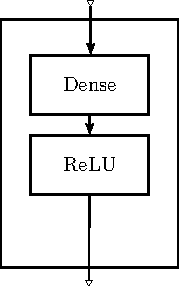
\includegraphics[scale=1]{theory/convergence-nonresidual-layer.pdf}
        \caption{Traditional Dense-ReLU layer}
    \end{subfigure}
    ~ %
    \begin{subfigure}[b]{0.4\textwidth}
        \centering
        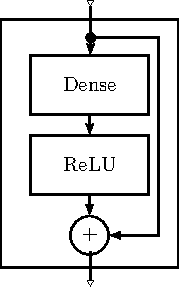
\includegraphics[scale=1]{theory/convergence-residual-layer.pdf}
        \caption{Residual Dense-ReLU layer}
    \end{subfigure}
    \caption{Comparetion of traditional and residual Dense-ReLU layer}
\end{figure}

The idea is that getting $\mathcal{F}(\mathbf{x}) = 0$ is a lot easier to solve than $\mathcal{H}(\mathbf{x}) = \mathbf{x}$. For both the ReLU and sigmoid transformation, $\mathcal{F}(\mathbf{x}) = 0$ can be obtained by moving the weights to some extreme, while $\mathcal{H}(\mathbf{x}) = \mathbf{x}$ is drastically more difficult, particularly for the sigmoid case. If the layer really needs a non-trivial $\mathcal{H}(\mathbf{x})$ function, the optimizer simply needs to find $\mathcal{H}(\mathbf{x}) - \mathbf{x}$, which should not be that much more difficult.

A downside of using a residual layer is that the output dimention must match the dimention of $\mathbf{x}$. However there are workarounds, for example one can add an extra dense layer to change the dimentionality of either the output dimention or $\mathbf{x}$.